\section{Experimental Evaluation}
\label{sec:evaluation}

The evaluation asks whether the candidate is useful before exact repair and whether machine learning improves that candidate enough to justify its cost. We therefore measure the proposed explanation separately from the exact result. The experiments progress from controlled test families to larger synthetic Petri nets, competing approximations, and real event logs. This order separates the effects of semantic constraints, learned ranking, representation, and input scale.

\subsection{Protocol, Metrics, and Comparison Boundaries}
\label{sec:protocol}

The reference experiments use an Intel Core i7-1355U CPU and the approximately 1.7-million parameter checkpoint selected at epoch 49. Computation is CPU only, with PyTorch reporting ten intra operation and ten inter operation threads; trace calls are sequential. The checkpoint is loaded once before timing. The synthetic test set has 512 rows from 128 generated families, with 64 rows for each motif/representation cell. The scoring parameters stay fixed throughout the test, scaling, and real log experiments.

The primary metrics are replay acceptance, exact cost agreement, and the cost gap in Equation~\eqref{eq:gap}. We also report full transition aware move sequence agreement with the teacher and agreement after replacing transition identities with labels. These sequence measures diagnose imitation of one witness; neither is required for an optimum when several witnesses share its cost. For representation pairs, cost agreement measures whether the same observation receives equal candidate costs on the two equivalent Petri nets.

The guidance ablation preserves the decoder, costs, depth bounds, and test inputs. It disables the neural forward pass and uses deterministic orderings in place of learned rankings. This is a strong baseline because enabledness and bounded model path search already resolve many cases. It directly answers RQ2; comparison with exact search alone would not isolate the contribution of machine learning.

For the LARA timing measurements, fast mode latency includes feature extraction, runtime construction, neural inference when enabled, decoding, and replay. Exact timings include the PM4Py heuristic initialization and search. In the approximation benchmark, the stored timing surrounds the PM4Py alignment call; independent parsing and replay occur afterward. These boundaries are not identical, so small timing differences should not be overinterpreted. All candidate costs are nevertheless compared after replay under the same unit visible deviation policy. Reported medians describe the recorded runs, not a universal hardware independent threshold.

The default test decoder uses catch up depth eight and completion depth 32. Scaling and real log scripts use completion depth 64 while keeping the catch up depth at eight. Exact timeouts in the stress benchmark are 30 seconds, and approximation calls receive five seconds. A timeout leaves the exact cost unknown; the corresponding candidate is included in coverage statistics but excluded from cost gap and optimality calculations that require the optimum. The tables state these denominators explicitly.

For representation specific guidance differences, a family bootstrap constructs 10,000 resampled datasets by drawing whole families with replacement, using seed 13 to make the random draws reproducible. The 2.5th and 97.5th percentiles of the resampled differences define the reported 95\% intervals. A cell contains 32 families with two observations each. Resampling families respects the dependence between observations and representations. These intervals describe sampling within the fixed generator and checkpoint; they do not include variability from retraining with different seeds.

\subsection{Candidate Quality on the Synthetic Test Split}
\label{sec:indist}

The first experiment answers whether the fast pipeline produces complete executable explanations and how close they are to the optimum (RQ1). All 512 candidates pass independent replay. Of these, 466 have the exact optimal cost, giving 91.0\% optimality. Table~\ref{tab:headline} reports the remaining diagnostics and Figure~\ref{fig:gaps} shows the full gap distribution.

\begin{table*}[!t]
\caption{Candidate results on the 512-row synthetic test split. Exact costs come from the teacher/reference alignment; candidate metrics precede any exact repair.}
\label{tab:headline}
\centering
\begin{tabularx}{\linewidth}{@{}Yr@{}}
\toprule
Metric & Result\\
\midrule
Candidate verified by replays & 512/512 (100.0\%)\\
Candidates with optimal cost & 466/512 (91.0\%)\\
Full transition aware move sequence match & 313/512 (61.1\%)\\
Full label level move sequence match & 320/512 (62.5\%)\\
Mean / median cost gap & 0.180 / 0\\
90th / 95th percentile cost gap & 0 / 2\\
Maximum cost gap & 4\\
\bottomrule
\end{tabularx}
\end{table*}

\begin{figure*}[!t]
\centering
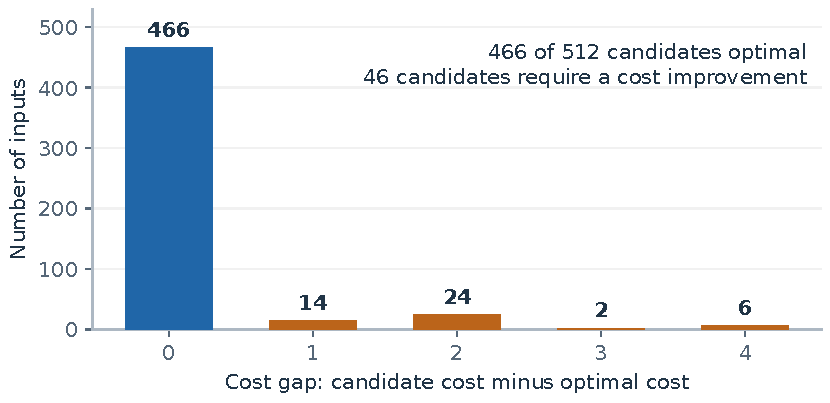
\includegraphics[width=\linewidth]{figures/cost_gaps.pdf}
\caption{All candidate gaps on the test split. Counts sum to 512; 466 candidates have gap zero and 46 have positive gaps. A low mean gap does not make a particular unchecked candidate optimal.}
\label{fig:gaps}
\end{figure*}

The mean gap is small because most candidates are optimal and the remaining gaps are between one and four. Sequence agreement is substantially lower than cost agreement. This is expected when several legal explanations are optimal and the teacher stores one of them. The important distinction for the assurance contract is that replay proves feasibility while exact cost comparison proves optimality, regardless of identity agreement.

When certified mode is evaluated on these inputs, it invokes exact search on all 512. The 466 optimal candidates can be confirmed and retained; the remaining 46 are replaced by exact alignments. The 91.0\% value therefore counts successful proposals, not traces on which exact search was avoided. This experiment establishes useful candidate quality within the generator, while leaving end to end certification acceleration unproven.

\subsection{What Does Learned Guidance Add?}
\label{sec:ablation}

The ablation isolates learned ranking from the model semantics. Unguided decoding also returns 512 legal candidates and reaches optimal cost on 445 of them, or 86.9\%. Adding the learned scorer yields 21 more optimal candidates, an increase of 4.10 percentage points. Mean gap decreases from .258 to .180. Transition aware sequence agreement rises from 57.8\% to 61.1\%, and label level agreement from 58.8\% to 62.5\%.

These aggregate gains are real for the fixed test set but do not imply that machine learning is responsible for most successful alignments. The unguided decoder already synchronizes uniquely enabled matches and searches for short model move paths. Many inputs offer little meaningful ranking choice. To answer where the improvement comes from, Table~\ref{tab:classes} separates the eight representation cells and Figure~\ref{fig:guidance} shows the corresponding differences.

\begin{table*}[!t]
\caption{Optimality by motif and representation. Each cell contains 64 inputs. G and U identify guided and unguided decoding; all outputs pass replay. Mean gaps are reported for guided candidates.}
\label{tab:classes}
\centering
\begin{tabularx}{\linewidth}{@{}lYrrr@{}}
\toprule
Motif & Representation & G optimal & U optimal & G mean gap\\
\midrule
Ordinary tree & Canonical block & 54/64 (84.4\%) & 55/64 (85.9\%) & .344\\
Ordinary tree & Isomorphic rename & 54/64 (84.4\%) & 49/64 (76.6\%) & .344\\
Duplicate/silent & Duplicate prefix & 61/64 (95.3\%) & 44/64 (68.8\%) & .094\\
Duplicate/silent & Silent routing & 63/64 (98.4\%) & 63/64 (98.4\%) & .031\\
Concurrency & Parallel & 58/64 (90.6\%) & 58/64 (90.6\%) & .219\\
Concurrency & Interleaving & 58/64 (90.6\%) & 58/64 (90.6\%) & .219\\
M pattern & Canonical block & 59/64 (92.2\%) & 59/64 (92.2\%) & .094\\
M pattern & Non-free choice & 59/64 (92.2\%) & 59/64 (92.2\%) & .094\\
\bottomrule
\end{tabularx}
\end{table*}

\begin{figure*}[!t]
\centering
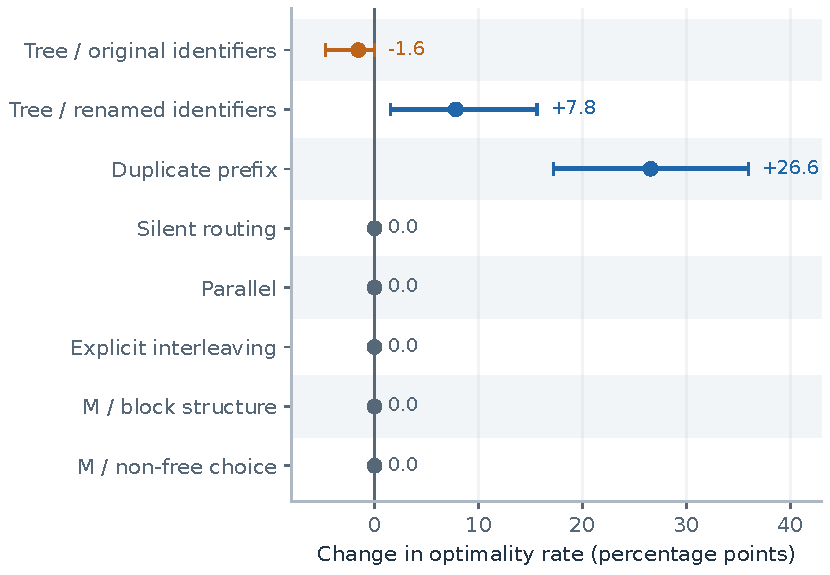
\includegraphics[width=\linewidth]{figures/guidance_effect.pdf}
\caption{Change in optimality rate when the fixed scorer is enabled. Positive values favor guidance. Intervals are 95\% percentile intervals from 10,000 family level bootstrap resamples; the zero width intervals indicate identical sampled success differences, not certainty about other generators. The strongest gain is concentrated in duplicate prefix choices.}
\label{fig:guidance}
\end{figure*}

The duplicate prefix cell improves from 68.8\% to 95.3\%, a gain of 26.6 points, with a family bootstrap interval of $[17.2,35.9]$ points. This is the case in which the trace suffix can distinguish two currently enabled transitions with the same label. Silent routing already attains 98.4\% without machine learning: its bounded search can postpone the choice until the distinguishing event. Guided and unguided costs coincide on the parallel/interleaving and M cells. RQ2 therefore has a localized answer: the measured gain is strongest where the decoder must commit before structural enabledness resolves the ambiguity.

\subsection{Sensitivity to Equivalent Representations}
\label{sec:representations}

Equivalent models let us examine reuse without changing the visible alignment problem (RQ3). Table~\ref{tab:pairagreement} compares candidate costs across each representation pair for the same observation. The ordinary tree pair is particularly informative because the two Petri nets differ only in identifiers.

\begin{table*}[!t]
\caption{Candidate cost agreement across paired representations. Each row compares 64 observation pairs. Exact costs agree in every pair. Candidate cost equality may include two equally suboptimal results.}
\label{tab:pairagreement}
\centering
\begin{tabularx}{\linewidth}{@{}Yrr@{}}
\toprule
Equivalent representation pair & Guided agreement & Unguided agreement\\
\midrule
Canonical tree / isomorphic rename & 100.0\% & 90.6\%\\
Duplicate prefix / silent routing & 96.9\% & 70.3\%\\
Parallel / explicit interleaving & 100.0\% & 100.0\%\\
Block M / non-free-choice M & 100.0\% & 100.0\%\\
\midrule
All 256 observation pairs & 99.2\% & 90.2\%\\
\bottomrule
\end{tabularx}
\end{table*}

Guided decoding reaches 84.4\% optimality on both canonical and renamed trees, with identical paired costs. Unguided decoding falls from 85.9\% to 76.6\% after renaming. Guidance is thus slightly worse on canonical identifiers, by $-1.6$ points with interval $[-4.7,0.0]$, but better on the renamed identifiers by $+7.8$ points with interval $[1.6,15.6]$. These signs have a common explanation: deterministic name order happens to be favorable on one numbering and less favorable on the other. The learned scorer maintains the same quality across this tested renaming.

Across all representation pairs, agreement rises from 90.2\% to 99.2\%. This is evidence of stability for the tested transformations, not proof of invariance under every isomorphism or activity relabeling. Ties, numerical behavior, and changed label embeddings can still affect choices. It also does not establish transfer to unseen compilation schemes: all four representation families occur during training.

\subsection{Scaling: Candidate Latency and Quality Together}
\label{sec:scaling}

The scaling experiment tests whether the candidate remains useful when inputs move beyond the small training distribution. A separate generator produces random block structured Petri nets with sequence, choice, parallelism, loops, duplicate labels, and invisible routing. The nominal sizes are 5, 10, 20, and 40 visible leaf occurrences. An alphabet fraction of .7 permits repeated labels; loop playout uses redo probability .3 and at most two redos. Deviations are injected at rates .15 and .35, with ten inputs per configuration. These rates are parameters of the stress generator, not the clean/noisy mixture in Section~\ref{sec:corruption}. Table~\ref{tab:scaling} reports the sizes, quality measures, and timings for all eight configurations.

\begin{table*}[!t]
\caption{Scaling results. Size is the requested visible leaf count and $\overline{|T|}$ the rounded mean total transition count. Every configuration has ten legal candidates. $n_\delta$ is the number with an exact reference; optimality and mean gap use that denominator. Time columns are median milliseconds per trace; exact timeouts are recorded at 30 seconds.}
\label{tab:scaling}
\centering
\begin{tabular}{@{}rrrrrrrr@{}}
\toprule
Size & Deviation & $\overline{|T|}$ & $n_\delta$ & Optimal & Mean gap & Fast ms & Exact ms\\
\midrule
5 & .15 & 7 & 10 & 90.0\% & .2 & 5.5 & 1.3\\
5 & .35 & 6 & 10 & 60.0\% & 1.6 & 4.6 & 1.3\\
10 & .15 & 13 & 10 & 80.0\% & 1.2 & 5.0 & 1.8\\
10 & .35 & 13 & 10 & 50.0\% & 1.7 & 5.3 & 2.8\\
20 & .15 & 28 & 10 & 60.0\% & 3.6 & 6.9 & 2.9\\
20 & .35 & 26 & 10 & 60.0\% & 3.1 & 6.0 & 11.7\\
40 & .15 & 55 & 10 & 30.0\% & 8.1 & 8.7 & 63.9\\
40 & .35 & 54 & 9 & 44.4\% & 11.7 & 8.6 & 24.7\\
\bottomrule
\end{tabular}
\end{table*}

\begin{figure*}[!t]
\centering
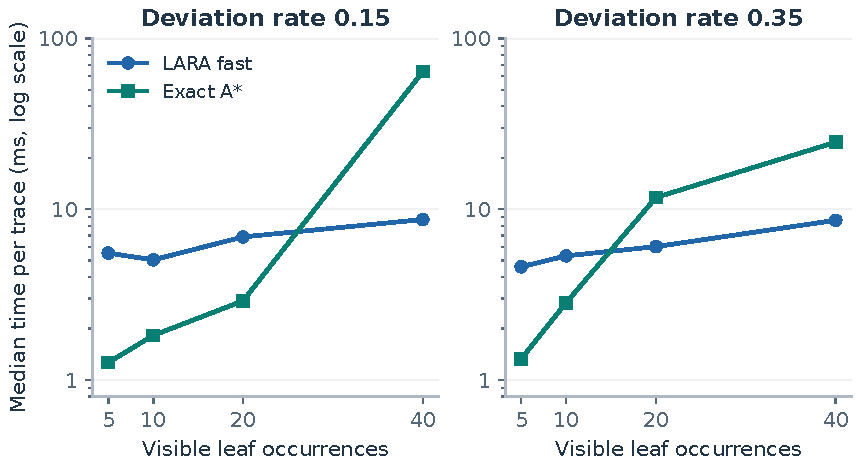
\includegraphics[width=\linewidth]{figures/scaling_latency.pdf}
\caption{Recorded median latencies on the scaling grid. The vertical axis is logarithmic; the horizontal axis is the number of visible leaf occurrences, not distinct activity labels. Exact search is faster on smaller cells, while its median is larger on several larger cells. These observations do not establish an asymptotic runtime law.}
\label{fig:scalingtime}
\end{figure*}

Figure~\ref{fig:scalingtime} compares the median latencies across this grid. LARA's guided median ranges from 4.6 to 8.7 ms. Exact A* is faster on the small configurations. It becomes slower at size 20 with deviation .35, and at size 40 for both rates. At size 40 and deviation .15 the median ratio is approximately $63.9/8.7=7.34$ in favor of the fast candidate. One exact call times out at size 40 and deviation .35. These are candidate latency comparisons, not certified mode speedups.

\begin{figure*}[!t]
\centering
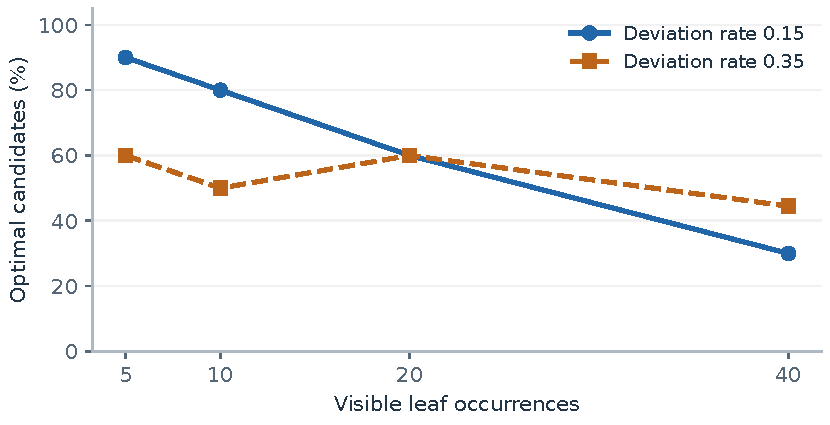
\includegraphics[width=\linewidth]{figures/scaling_quality.pdf}
\caption{The quality cost of the latency advantage in Figure~\ref{fig:scalingtime}. Optimality declines on larger stress inputs. Each point uses ten exact references except size 40/deviation .35, which uses nine. Small cell sizes and changing random Petri nets explain why the curves need not be monotone.}
\label{fig:scalingquality}
\end{figure*}

Figure~\ref{fig:scalingquality} shows the accompanying decline in quality: at size 40 only 30.0\% or 44.4\% of comparable candidates are optimal, and mean gaps reach 8.1 or 11.7. Replay remains successful on all 80 candidates, demonstrating executability despite this loss of quality. Unguided decoding takes approximately .2--1.2 ms across the grid and is faster than the exact medians throughout. Guidance contributes little on this stress distribution. The practical question is therefore whether better rankings justify the neural inference cost, not simply whether a neural forward pass is faster than a difficult exact search.

\subsection{Comparison with Established Approximations}
\label{sec:approximations}

Competing candidate generators provide a more demanding test than exact search alone. The benchmark uses PM4Py 2.7.23.2 implementations of discounted A*~\cite{Boltenhagen2021}, tandem repeats~\cite{ReissnerTandem2020}, sliding windows~\cite{Bogdanov2024}, fixed horizon search~\cite{Dongen2017}, and subset/edit distance approximation~\cite{FaniSani2020}. Sliding windows use length 20 and at most five candidates; the fixed horizon is four; the configured expansion budget is 100,000 where supported. The subset size is one within each model variant group and is evaluated only on the test corpus. These are concrete settings, not tuned best case envelopes for each method.

All returned alignments are parsed into transition aware moves, replayed independently, and rescored with the same costs. This is particularly important for discounted objectives: their internally reported objective need not equal the ordinary visible deviation count. Table~\ref{tab:approxsmall} reports the test comparison, and Table~\ref{tab:approxstress} reports stress results from the approximation benchmark run.

\begin{table*}[!t]
\caption{Candidate quality on the synthetic test split. All six methods provide 512 legal outputs in this experiment, so the optimality denominator is 512 for every row.}
\label{tab:approxsmall}
\centering
\begin{tabularx}{\linewidth}{@{}Yrr@{}}
\toprule
Method & Optimal candidates & Mean gap\\
\midrule
LARA guided & 466/512 (91.0\%) & .180\\
Discounted A* & 490/512 (95.7\%) & .090\\
Tandem repeats & 502/512 (98.0\%) & .039\\
Sliding window & 512/512 (100.0\%) & .000\\
Fixed horizon & 502/512 (98.0\%) & .047\\
Subset/edit distance & 360/512 (70.3\%) & .637\\
\bottomrule
\end{tabularx}
\end{table*}

Every tested Petri net search/compression approximation exceeds LARA's optimality rate on the small corpus. LARA exceeds the particular subset/edit distance configuration. All test traces fit within one sliding window of 20 events, so the perfect result in that row does not exercise the approximation caused by crossing a window boundary. The comparison illustrates why a small benchmark can be useful for diagnosis without being a sufficient stress test.

\begin{table*}[!t]
\caption{Stress comparison over 80 inputs. Coverage counts legal outputs out of all 80; $n_\delta$ counts legal outputs with an exact reference. Optimality and mean gap are conditional on those $n_\delta$ inputs. Time is the median over all calls, including unsuccessful calls. Different coverage denominators limit direct quality comparisons.}
\label{tab:approxstress}
\centering
\begin{tabularx}{\linewidth}{@{}Yrrrrr@{}}
\toprule
Method & Coverage & $n_\delta$ & Optimal & Mean gap & Median ms\\
\midrule
LARA guided & 80/80 & 79 & 59.5\% & 3.797 & 7.69\\
Discounted A* & 80/80 & 79 & 75.9\% & 1.468 & 1.17\\
Tandem repeats & 78/80 & 78 & 93.6\% & .128 & 1.37\\
Sliding window & 79/80 & 79 & 100.0\% & .000 & 1.27\\
Fixed horizon & 76/80 & 76 & 82.9\% & 2.263 & 82.37\\
\bottomrule
\end{tabularx}
\end{table*}

The stress comparison again favors established approximations in quality. Discounted A* has the same full legal coverage as LARA, a higher exact cost rate, a smaller mean gap, and a lower recorded median latency. Tandem repeats and sliding windows are even closer to optimal where they return comparable results. Their incomplete coverage must remain visible: a perfect conditional optimum rate is not a result on every attempted input. LARA's full coverage is useful, but it is not unique to the learned method on this grid.

The small and stress comparisons rule out a claim that the present learned greedy decoder is the best general approximation. They instead identify a reusable scoring mechanism with a measured local advantage over its own unguided baseline. Any later claim of competitive overall approximation quality requires a stronger decoder and renewed comparison using common timing boundaries and coverage accounting.

\subsection{Application to Public Event Logs without Fine Tuning}
\label{sec:real}

Real log inputs test the use of one checkpoint with different vocabularies, model structures, and trace lengths. We use a building permit receipt log~\cite{ReceiptLog}, containing 1434 cases, 116 variants, and 27 activity labels, and the repository's 100-case sample of the road traffic fines log~\cite{RoadTrafficLog}, containing ten variants and ten labels. The road traffic results refer to that sample, not the complete public log. The longest variants have 25 and nine events, respectively.

For each log, PM4Py discovers Petri nets using Inductive Miner~\cite{Leemans2013} at noise threshold .0 and its infrequent behavior variant~\cite{Leemans2014} at threshold .5. Models are discovered from the same log that is subsequently aligned, so this experiment evaluates algorithmic transfer, not independent normative compliance. The positive noise threshold removes infrequent behavior and creates additional deviations against the resulting model. The checkpoint is unchanged; new label strings enter through hashing without any language interpretation or fine tuning.

\begin{table*}[!t]
\caption{Real log candidate quality. All variants pass replay. Petri net size gives places and visible/invisible transitions. Guided and unguided decoding have identical quality values in all four configurations. Mean and maximum gaps are over variants.}
\label{tab:realquality}
\centering
\begin{tabular}{@{}llrrrr@{}}
\toprule
Log & Noise & Petri net size & \multicolumn{2}{c}{Optimal (\%)} & Gap\\
 & & $|P|/|T_v|+|T_\tau|$ & Variants & Cases & Mean/max\\
\midrule
Road traffic & .0 & $15/10+10$ & 100.0\% & 100.0\% & 0/0\\
Road traffic & .5 & $13/10+7$ & 70.0\% & 94.0\% & .50/3\\
Receipt & .0 & $45/27+47$ & 50.0\% & 82.6\% & .76/5\\
Receipt & .5 & $25/24+19$ & 55.2\% & 74.6\% & .82/7\\
\bottomrule
\end{tabular}
\end{table*}

Table~\ref{tab:realquality} distinguishes variants from cases. If variant $v$ occurs $f_v$ times, case weighted optimality is
\begin{equation}
 \frac{\sum_v f_v\ind[g_v=0]}{\sum_vf_v},
 \label{eq:weighted}
\end{equation}
whereas variant optimality weights each distinct sequence once. The higher case weighted values show that frequent variants are easier for this decoder; misses are concentrated in less frequent variants. For the fitting receipt Petri net, all exact costs are zero, but only half of the candidate variants attain zero. A legal, positive cost candidate on a fitting trace is therefore a concrete example of why replay alone is insufficient to infer nonconformance.

\begin{table*}[!t]
\caption{Recorded median time per variant in milliseconds. These are candidate/exact timings, not full log wall clock speedups. Including the unguided decoder makes clear that the real log candidate advantage is not evidence of a learned quality benefit.}
\label{tab:realtime}
\centering
\begin{tabularx}{\linewidth}{@{}Yrrrr@{}}
\toprule
Log & Noise & Guided fast & Unguided fast & Exact A*\\
\midrule
Road traffic & .0 & 5.39 & .56 & 1.92\\
Road traffic & .5 & 5.22 & .48 & 1.56\\
Receipt & .0 & 16.05 & 6.01 & 31.04\\
Receipt & .5 & 6.65 & .61 & 12.72\\
\bottomrule
\end{tabularx}
\end{table*}

The guided candidate is slower than exact search on the small road traffic Petri nets and faster on the tested receipt Petri nets (Table~\ref{tab:realtime}). Unguided decoding is faster still and has the same candidate quality. These discovered Petri nets have no duplicate visible labels, so they do not exercise the scorer's strongest demonstrated advantage. Model move ordering could still matter in principle, but no quality difference is observed here. The experiment supports interface transfer and verified execution under different inputs; it does not demonstrate that the neural scorer improves real log alignment quality.

\subsection{A Failure That Explains the Remaining Gaps}
\label{sec:failure}

Aggregate rates show how often the decoder fails to be optimal; the worked failure in Figure~\ref{fig:failure} explains why. Consider test observation $\langle A,D,B,C,C,D\rangle$ in the parallel/interleaving family. Its process permits $A,B$ in either order, then $C,D$. An optimal alignment skips the early $D$ and one repeated $C$, giving cost two. LARA instead inserts model moves $B,C$ so that it can synchronize the early $D$. It reaches the final marking while four observed events remain, forcing four log moves. Its total cost is six, hence gap four.

\begin{figure*}[!t]
\centering
\begin{tikzpicture}[x=1cm,y=1cm]
\node[paneltitle] at (0,.95) {A. Skip the early $D$ and one repeated $C$};
\node[annotation,anchor=east] at (1,0) {log};
\node[annotation,anchor=east] at (1,-.7) {model};
\foreach \x/\l/\m in {1.7/A/A,3.9/B/B,5/C/C,7.2/D/D}{
\node[alcell] at (\x,0) {$\l$};\node[alcell] at (\x,-.7) {$\m$};}
\foreach \x/\l in {2.8/D,6.1/C}{
\node[devcell] at (\x,0) {$\l$};\node[devcell] at (\x,-.7) {$\skipmove$};}
\node[verifybox,text width=16mm] at (9.35,-.35) {optimal\\cost $2$};
\node[annotation,anchor=west] at (1.15,-1.4) {4 synchronous moves + 2 log moves};
\node[paneltitle] at (0,-2.35) {B. Catch up to the early $D$, then finish too soon};
\node[annotation,anchor=east] at (1,-3.3) {log};
\node[annotation,anchor=east] at (1,-4) {model};
\foreach \x/\l/\m in {1.7/A/A,5/D/D}{
\node[alcell,fill=softblue] at (\x,-3.3) {$\l$};\node[alcell,fill=softblue] at (\x,-4) {$\m$};}
\foreach \x/\m in {2.8/B,3.9/C}{
\node[devcell] at (\x,-3.3) {$\skipmove$};\node[devcell] at (\x,-4) {$\m$};}
\foreach \x/\l in {6.1/B,7.2/C,8.3/C,9.4/D}{
\node[devcell] at (\x,-3.3) {$\l$};\node[devcell] at (\x,-4) {$\skipmove$};}
\draw[devamber,line width=1pt] (2.25,-4.55) -- (4.45,-4.55);
\draw[devamber,line width=1pt] (5.55,-4.55) -- (9.95,-4.55);
\node[annotation,text=devamber] at (3.35,-4.95) {2 model moves};
\node[annotation,text=devamber] at (7.75,-4.95) {4 log moves after completion};
\node[warnbox,text width=100mm] at (5.5,-6) {Candidate cost $2+4=6$; optimal cost $2$; gap $4$.\\Every firing is legal, but the early decision harms the suffix.};
\end{tikzpicture}

\caption{A legal but suboptimal explanation of $\langle A,D,B,C,C,D\rangle$. Each visible deviation is amber. Invisible routing is omitted, and model rows display activity labels for readability. The upper explanation costs two; the lower costs six. The early attempt to synchronize $D$ causes both the two inserted model activities and the four subsequent skipped events.}
\label{fig:failure}
\end{figure*}

The error is a decoder commitment, not a replay failure. The decoder tries a bounded model path before considering a log move and never compares that path with skipping the early $D$. The trained log score is unused, and earlier choices cannot be revised. Better duplicate label scoring cannot fix every instance of this mechanism. It motivates joint ranking of synchronous, log, and model alternatives and retaining several candidate continuations, as discussed next.
